\chapter{Executive summary}
\label{ch:fdsp-execsum}

\section{Introduction}
\label{sec:fdsp-exec-introduction}
%Broad physics motivation for the detector.


The overriding physics goals of DUNE are the search for leptonic CP violation, the observation of neutrinos bursts from supernovae, and the search for nucleon decay as a signature of a Grand Unified Theory underlying the Standard Model. Central to achieving this physics programme is the construction of a detector that combines the many-kiloton fiducial mass necessary for rare event searches with sub-centimetre spacial resolution in its ability to image those events, allowing us to identify the signatures of the physics processes we seek amongst the numerous backgrounds. The single-phase liquid-argon time-projection chamber (LArTPC)~\cite{ref:RubbiaLartpc} allows us to achieve these dual goals, providing a way to read out with sub-centimetre granularity the patterns of ionisation in $\SI{10}{kt}$ volumes of liquid argon resulting from the $O(\SI{1}{MeV})$ interactions of solar and supernova neutrinos up to the $O(\SI{1}{GeV})$ interactions of neutrinos from the LBNF beam.

To search for leptonic CP violation, we much search for \nue appearance in the LBNF \numu beam. This requires the ability to separate electromagnetic activity induced by charged-current \nue interactions from similar activity arising from photons, for example those from $\pi^{0}$ decay. Two signatures allow this: photon showers are preceded by a gap prior to the conversion of the photon, characterised by the \SI{14}{cm} conversion length; and the initial part of a photon shower has twice the $\mathrm{d}E/\mathrm{d}x$ of an electron-induced shower, clearly measurable given the signal-to-noise requirements on our ability to measure the ionisation of the argon. To search for proton decay, where the primary channel of interest is $p\rightarrow K^{+}\overline{\nu}$, we must identify kaon tracks as short as a few centimetres, which can be done thanks to the sub-\si{cm} spacial resolution of the LArTPC. It is also vital to accurately fiducialise these proton-decay events to suppress cosmic-muon-induced backgrounds, and here the detection of argon-scintillation photons is important. The detection of supernova neutrino bursts poses different challenges, those of data-rate and detector reliability. To fully reconstruct a supernova burst, the entire detector must be read out, at up to $\SI{2}{\tera\byte/\second}$, for \SIrange{30}{100}{s}, including a $\sim\!\SI{4}{s}$ pre-trigger window. And to ensure these rare events are not missed, all detector sub-systems must work together to ensure the highest live-time possible.

In what follows, we give an overview of the basic operating principles of a single-phase LArTPC, followed by a description of the DUNE implementation. We then discuss each of the sub-systems separately, connecting the high-level design requirements and decisions to the overriding physics goals of DUNE.

\section{The single-phase liquid-argon time-projection chamber}
\label{sec:fdsp-exec-splar}
%General operating principle

\begin{dunefigure}[The single-phase liquid-argon time-projection chamber]{fig:LArTPC}
{The general operating principle of the single-phase liquid-argon time-projection chamber.}
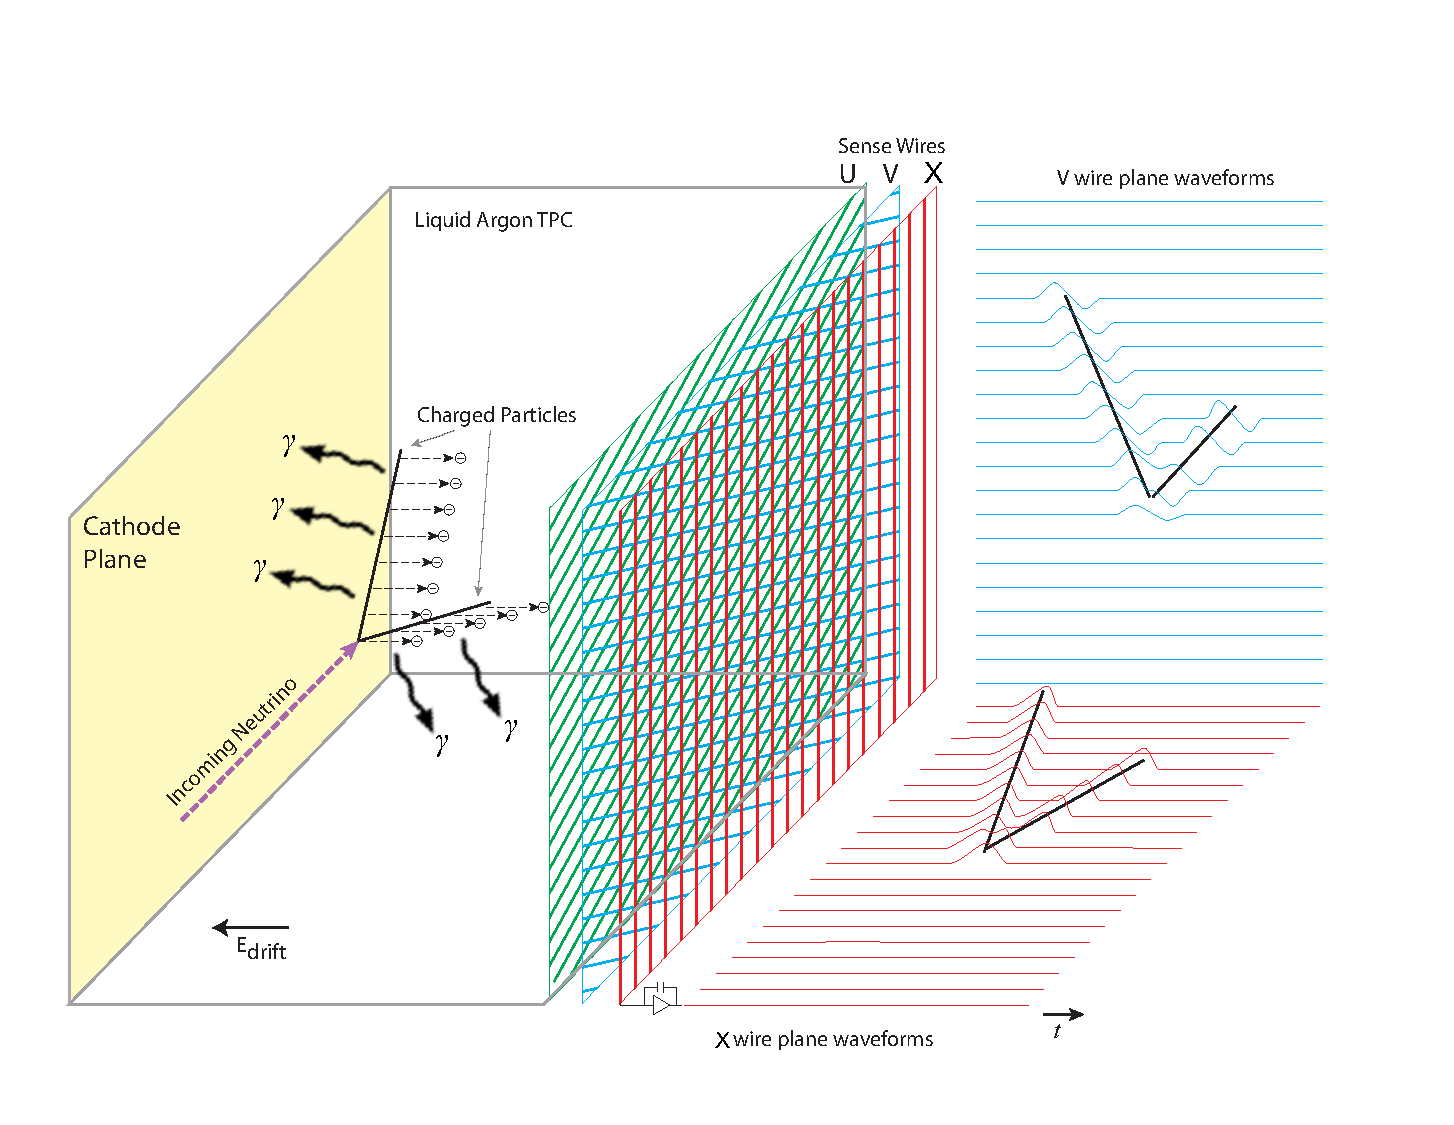
\includegraphics[width=0.8\textwidth]{LArTPC.pdf}
\end{dunefigure}

Figure~\ref{fig:LArTPC} shows the general operating principle of a single-phase LArTPC, as has been previously demonstrated by ICARUS~\cite{Icarus-T600}, MicroBooNE~\cite{ref:MicroBooNEDetectorPaper}, ArgoNeuT~\cite{Anderson:2012vc}, LArIAT~\cite{Cavanna:2014iqa} and ProtoDUNE~\cite{ref:ProtoDUNETDR}. A large volume of liquid argon is subjected to a strong electric field of a few hundred volts per centimetre. Charged particles passing through the detector ionise the argon, and the ionisation electrons drift in the electric field to the anodic wall over a period of $O(\SI{100}{\micro\second})$. This anode consists of three layers of active wires forming a grid. The relative voltage between the layers is chosen to ensure the first two layers are transparent to the drifting electrons, and these layers produce bipolar induction signals as the electrons pass through them. The final layer collects the drifting electrons, resulting in a monopolar signal. Liquid argon is also an excellent scintillator, at \SI{126.8}{\nano\meter}, and this fast scintillation light, once shifted into the visible, is collected by photon-detectors placed either in or near the anode plane.

The photon detectors provide a $t_{0}$ for every event, telling us when the ionisation electrons begin to drift. Relative to this $t_{0}$, the time at which the ionisation signal reaches the anode allows reconstruction of the event topology in the drift coordinate; the precision of this $t_{0}$ therefore directly corresponds to the precision of the spacial reconstruction in this direction. In addition to our ability to reconstruct topologies in the drift direction, this $t_{0}$ precision defines our ability to fiducialise proton-decay events and our ability to apply drift corrections to the ionisation charge.

The pattern of ionization collected on the grid of anode wires provides the reconstruction in the remaining two coordinates perpendicular to the drift direction. A closer spacing of the wires therefore results in better spacial resolution, however, as well as increasing the cost of the readout electronics due to the additional wire channels, a closer spacing worsens the signal-to-noise of the ionization measurement as the same amount of ionization charge is now being divided over more channels. Signal-to-noise is an important consideration since the measurement of the ionization collected is a direct measurement of the $\mathrm{d}E/\mathrm{d}x$ of the charged particles, and is what allows us to perform both calorimetry and particle identification.

\section{The DUNE singe-phase Far-Detector module}
\label{sec:fdsp-exec-dunefd}
%Explain 10 kt modules, and then explain the overall setup.
%As part of this, explain the main design parameters and how they relate to the physics drivers.

\begin{dunefigure}[A $\SI{10}{\kilo\tonne}$ DUNE Far Detector single-phase module.]{fig:DUNESchematic}
{A $\SI{10}{\kilo\tonne}$ DUNE Far Detector single-phase module, showing alternating anode (A) and cathode (C) planes.}
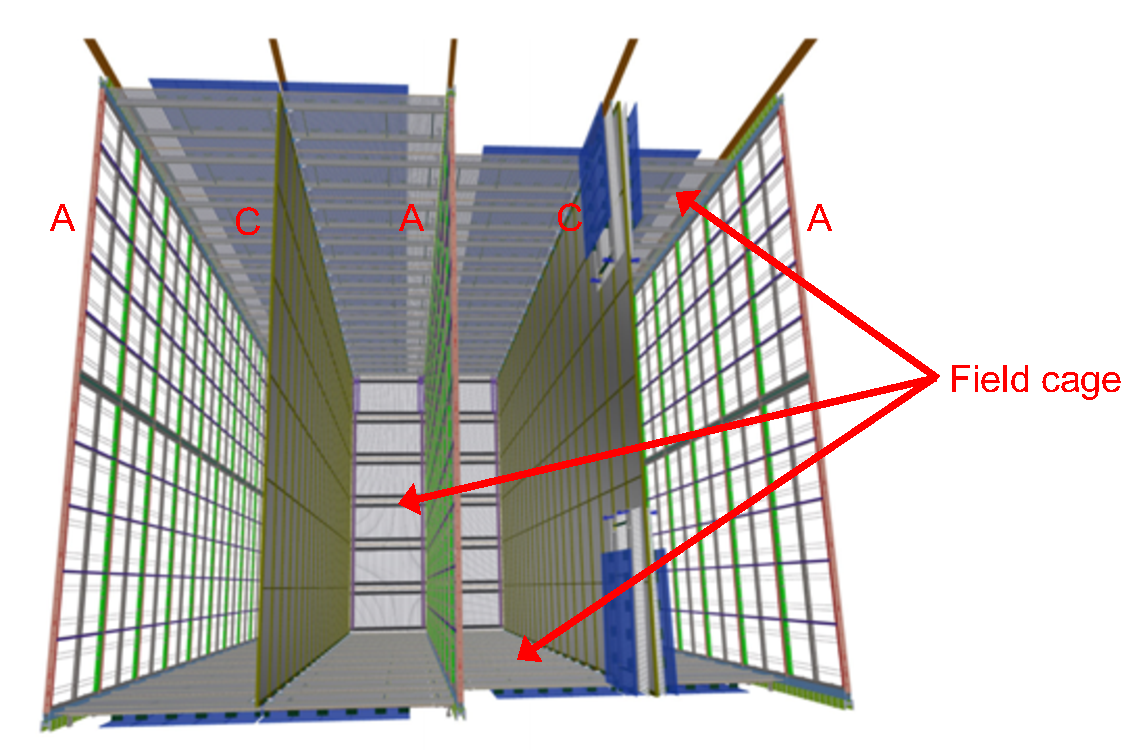
\includegraphics[width=0.8\textwidth]{DUNESchematic.pdf}
\end{dunefigure}

The DUNE single-phase LArTPC consists of \SI{10}{\kilo\tonne} modules, contributing to the full \SI{40}{\kilo\tonne} Far Detector fiducial mass. A \SI{10}{\kilo\tonne} module is shown in Figure~\ref{fig:DUNESchematic}. Inside a $x\times y \times z\,\si{\meter}$ cryostat, four $x\,\si{\meter}$ drift volumes are created between five alternating anodic and cathodic walls, each wall having dimensions of $x\times y\,\si{\meter}$.

Each $x\times y$\si{\meter} cathodic wall in a module is called a CPA array. The CPA (cathode plane assembly) is the $\SI{1.2}{\meter}\times\SI{2}{\meter}$ panel from which the CPA arrays are formed; each CPA array contains $x$ CPAs. These CPA arrays are held at $-\SI{180}{\kilo\volt}$. With the anodic walls held close to ground, this results in a \SI{500}{\volt/\centi\meter} drop across the drift volume. A field cage surrounds the remaining open sides of the TPC, ensuring the field is uniform to at least 1\% throughout the active volume. A typical minimum ionising particle passing through the argon produces around $60k$ ionisation electrons per centimetre, and these drift towards the anodes at around $x$\si{\meter/\micro\second}.

The $x\times y$\si{\meter} anode walls are each made up of 150 anode plane assemblies (APAs) of $\SI{6}{\meter}\times\SI{2.3}{\meter}$ in dimension. As can be seen in Figure~\ref{fig:APAStack} the APAs hang vertically, and each anode wall is two APAs high; the bottom APA hangs from the APA above it. The APAs are two-sided, with the three active wire layers, plus an additional shielding layer, wrapped around them. The collection layer is called the $x$-layer; the induction layer immediately next to that is called the $v$-layer; the next induction layer is the $u$-layer and the shielding layer is the $g$-layer. $x$-layer and $g$-layer wires are vertical; the $u$- and $v$-layer wires are at \SI{35.7}{\degree} to the vertical.

\begin{dunefigure}[A stack of two anode plane assemblies.]{fig:APAStack}
{I want this to be a picture of two APAs, mounted above each other, that shows the locations of the photon detectors and readout electronics.}
%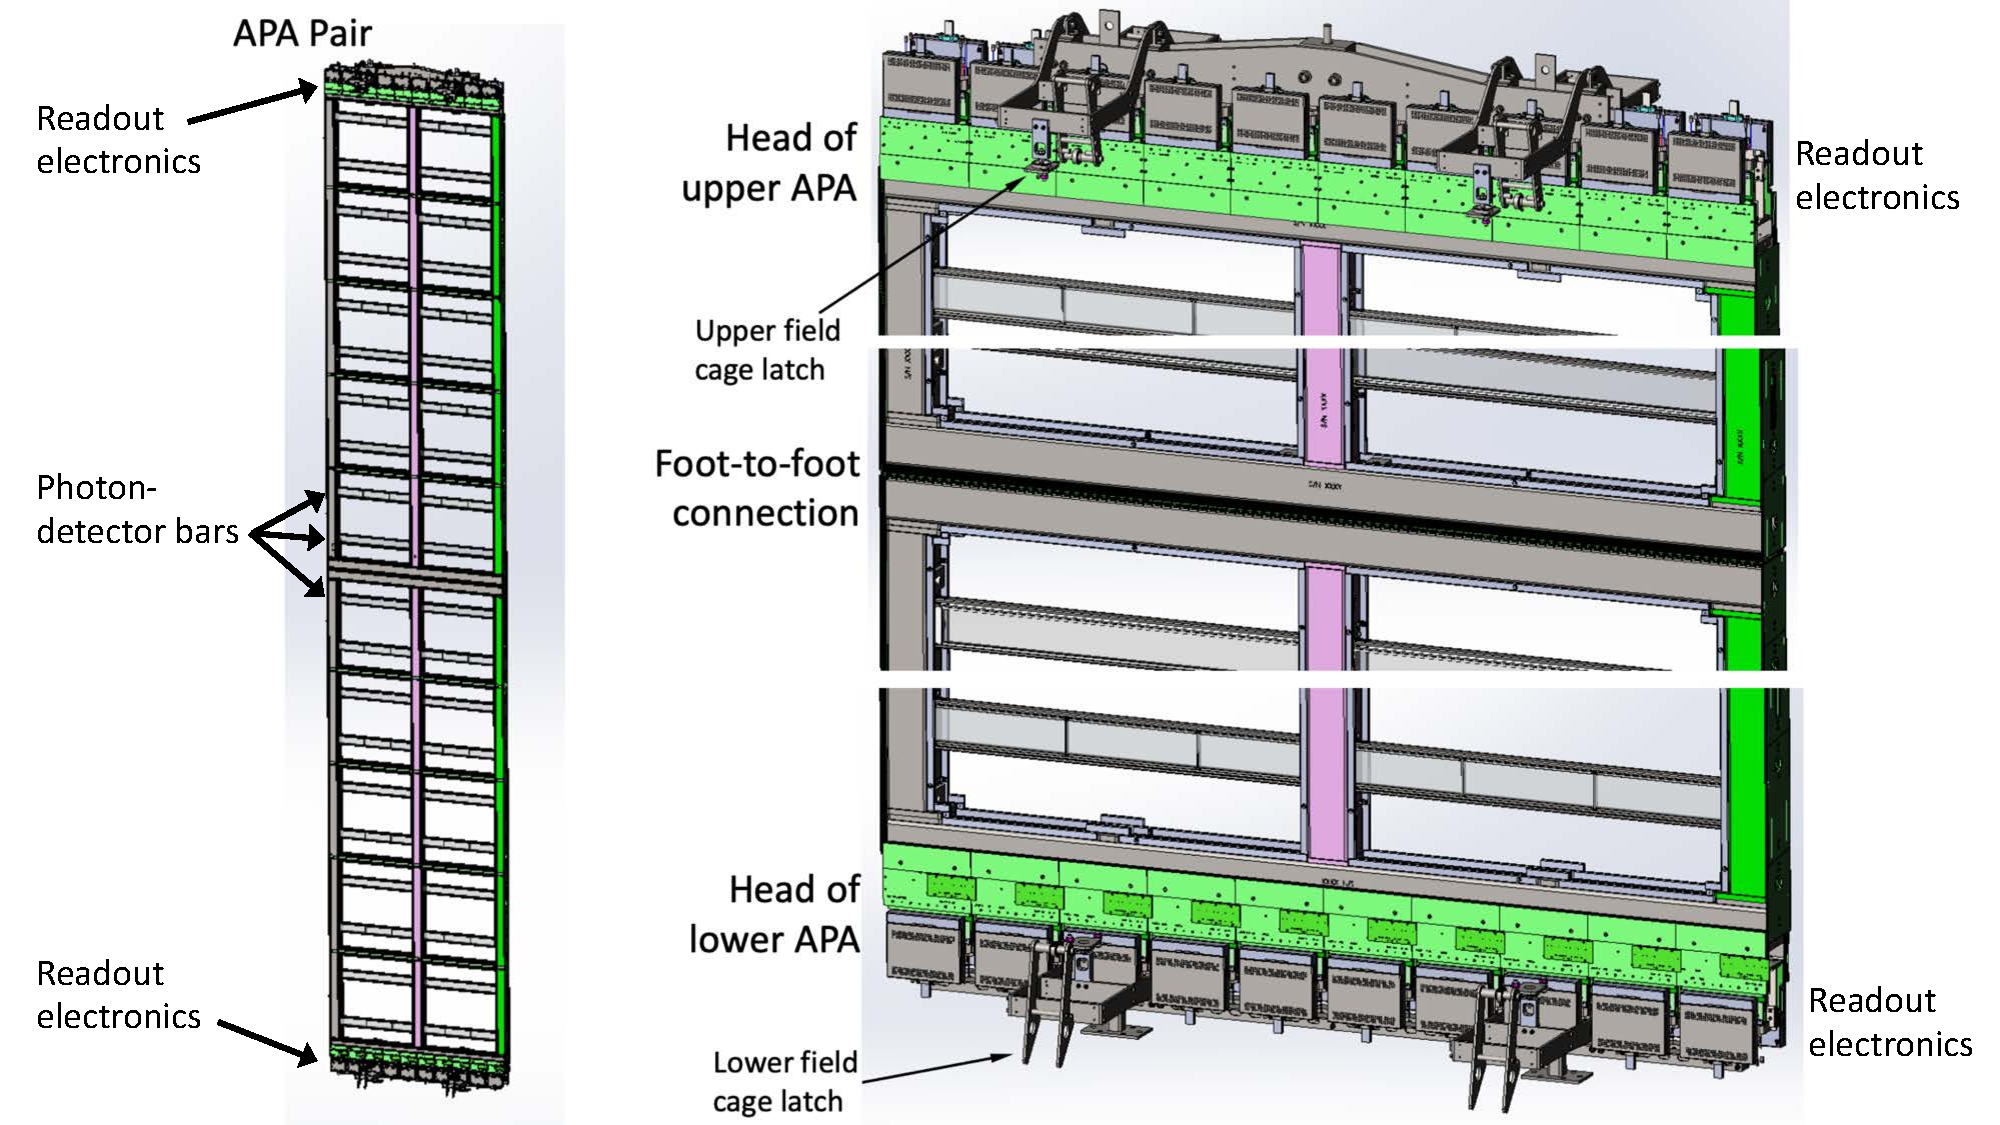
\includegraphics[width=0.8\textwidth]{Figures/APAStack.pdf}
\end{dunefigure}
\fixme{missing figure}

Readout electronics are attached to the APAs; the readout happens at the top end of the top APA and the bottom end of the bottom APA. These front-end electronics benefit from the liquid-argon temperatures through the reduction of thermal noise. The front-end electronics shape, amplify and digitize the signals from the induction and collection wires thanks to a series of three different types of ASIC through which all signals pass. On each APA there are 20 front-end motherboards, on which the ASICs are mounted, and each motherboard processes the signals from 40 $u$, 40 $v$ and 48 $x$-layer wires. Cables from the cold electronics pass through feedthroughs on the roof of the cryostat; cables from the motherboards on the bottom APA pass through the inside of the hollow APA frames to bring them up to the top.

Once the signals from the APAs leave the cryostat through the feedthroughs, they are passed to warm interface boards that put the signals onto \SI{10}{\giga\byte} optical fibres, ten fibres per APA, which carry the signals to the data-acquisition system that is located in the central utility cavern --- a cavern adjacent to the detector caverns underground. Each \SI{10}{\kilo\tonne} module has its own, independent data-acquisition system, built around the CERN-developed FELIX system, that is responsible for triggering, buffering, and shipping data out to permanent storage above ground; when triggered each \SI{10}{\kilo\tonne} module will provide data at a rate of up to \SI{2}{\tera\byte/\second}. This separation of data-acquisition systems allows each module to run as an independent detector to minimize the chance of a complete Far-Detector outage. There will, however, be the facility for modules to provide the others with a supernova trigger signal. The data-acquisition system also provides the detector clock. A GPS pps signal is used to time-stamp events, both to allow matching to the beam window and to allow time-stamping of supernova triggers. Within a \SI{10}{\kilo\tonne} module a $\SI{65}{\mega\hertz}$ master clock keeps all detector components synchronized to within \SI{1}{\nano\second}.

In addition to the ionisation, charged particles passing through the argon produce around 24,000 scintillation photons per \si{\mega\electronvolt}. These photons are collected by devices called X-Arapucas, which are mounted on the APAs, in between the two sets of wire layers, as shown in Figure~\ref{fig:APAStack}. There are ten X-Arapucas on each APA, which consist of $\SI{209.2}{\cm}\times\SI{11.8}{\cm}\times\SI{2.3}{\cm}$ bars, running the full \SI{2.3}{\meter} width of the APA. The X-Arapuca bars consist of layers of dichroic filter and wavelength-shifter that shift the \SI{126.8}{\nano\meter} light into the visible and trap these visible photons, transporting them to silicon photomultipliers (SiPMs). The signals from these SiPMs are sent along cables that pass through the hollow APA frames, up to feedthroughs in cryostat roof. The signals are then sent along \SI{10}{\giga\byte} optical fibres, one fibre per APA (ten X-Arapuca bars), to the DAQ system where the photon-detector and APA-wire data-streams are merged.

\section{The liquid argon}
\label{sec:fdsp-exec-liquidargon}

The primary requirement of the liquid argon is its purity. Electronegative contaminants such as oxygen or water will absorb ionisation electrons as they drift. Nitrogen contaminants will quench scintillation photons.

The target purity from electronegative contaminants in the argon is $<\!100$\,ppt O$_{2}$ equivalent, which is enough to ensure a $>\!\SI{3}{\milli\second}$ ionisation-electron lifetime at our nominal \SI{500}{\volt/\centi\meter} drift voltage. This target electron lifetime means that, for an ionisation event occurring near a CPA array, there is 48\% attenuation of the ionization by the time it reaches the anode, which ensures, for these events, that we still achieve our signal-to-noise requirements of $S/N>5$ for the induction planes and $S/N>10$
%COMMENT Are these two numbers both correct? The Induction >5 is definitely a requirement; the collection > 10 is also mentioned in passing in the cold-electronics chapter.
for the collection planes that govern our ability to perform pattern-recognition and two-track separation. We have an additional requirement on electronegative impurities released into the argon by detector components of $<\!30$\,ppt, to ensure such sources of contamination are negligible in comparison to the contamination inherent in the argon. Data from ProtoDUNE has shown that we can exceed our target argon purity, with electron lifetimes in excess of \SI{6}{\milli\second} achieved.

Nitrogen contamination is required to be $<\!25$\,ppm. This is necessary to ensure we achieve our requirement of at least 0.5 photoelectrons per MeV detected for events in all parts of the detector. This ensures, through the timing requirements discussed in section~\ref{sec:fdsp-exec-pds}, that we can fiducialize nucleon decay events throughout the detector.

The argon contains a natural $x$\% component of unstable $^{39}$Ar. This isotope undergoes $\beta$ decay, and these $\beta$-decay electron tracks, as well as the photons they produce, define the energy threshold below which we cannot trigger on low-energy physics events such as solar neutrinos without
%COMMENT give some number for photons produced by an Ar39 beta decay?
being swamped by background. We use this $^{39}$Ar contamination to form a requirement that all other detector components must introduce negligible radioactive contamination in comparison to the $^{39}$Ar.

Fundamental to maintaining the argon purity is the constant flow of argon through the purification system. It is therefore important to understand the fluid dynamics of the argon flow within the detector to ensure there are no `dead regions' where argon can become trapped. This fluid dynamics also informs the placement of purity, temperature and level monitors. The computational fluid dynamics, as well as the requirements on monitoring of the argon, and the instrumentation used to perform this monitoring, is described further in chapter~\ref{chap:fdsp-cisc}. 

%COMMENT Do I need a section on the other contents of the CISC chapter?

\section{Photon-detection system}
\label{sec:fdsp-exec-pds}

In comparison to the ionisation electrons, which can take milliseconds to drift across the drift volume, the scintillation photons are fast, arriving in nanoseconds. This fast scintillation light provides a $t_{0}$ for each event. By comparing the arrival time of ionisation at the anode with this $t_{0}$, reconstruction in the drift direction becomes possible. The spacial resolution of the detector perpendicular to the drift direction is defined by the $\sim\!\SI{5}{\mm}$ wire spacing on the APAs; a desire to achieve a comparable spacial resolution in the drift direction results in a \SI{1}{\micro\second} requirement on the timing resolution of the photon-detector system. Specifically, this requirement enables \SI{1}{\mm} position resolution for \SI{10}{\mega\electronvolt} supernova-burst events. The photon-detector $t_{0}$ is also vital in fiducialising nucleon-decay events, which allows us to reject cosmic-muon-induced background events that will occur near the edges of the detector modules. A requirement that we are able to do this throughout the entire active volume with $>\!99\%$ efficiency leads us to a requirement of at least 0.5 photoelectrons per MeV detected for events in all parts of the detector, which in turn requires an effective area of $\SI{23}{\cm^{2}}$ for each photon-detector module.


\begin{dunefigure}[Photon-detector modules, mounted in an anode pane assembly.]{fig:PDModules}
{Left: a photon-detector module. Right: a photon-detector module mounted in an APA.}
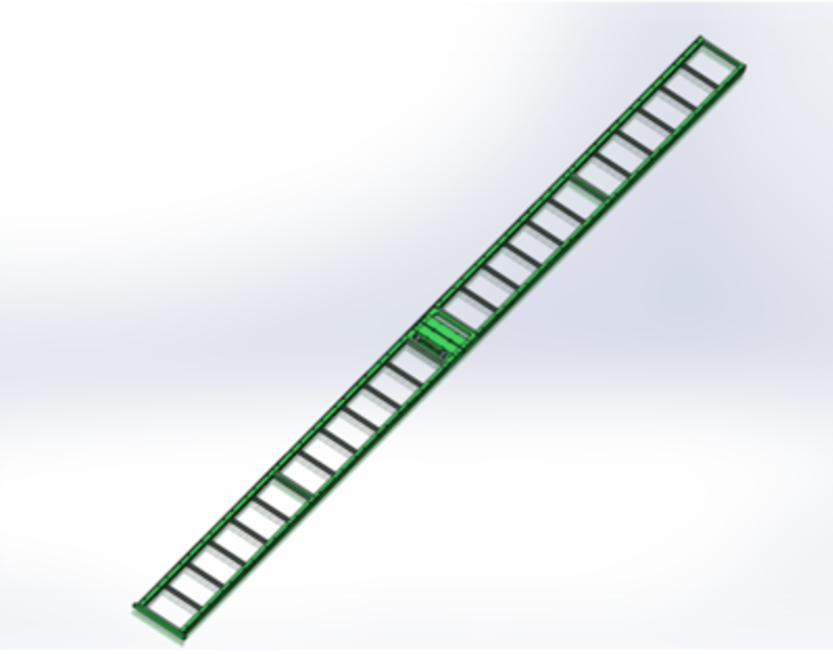
\includegraphics[width=0.49\textwidth]{PDBar.pdf}
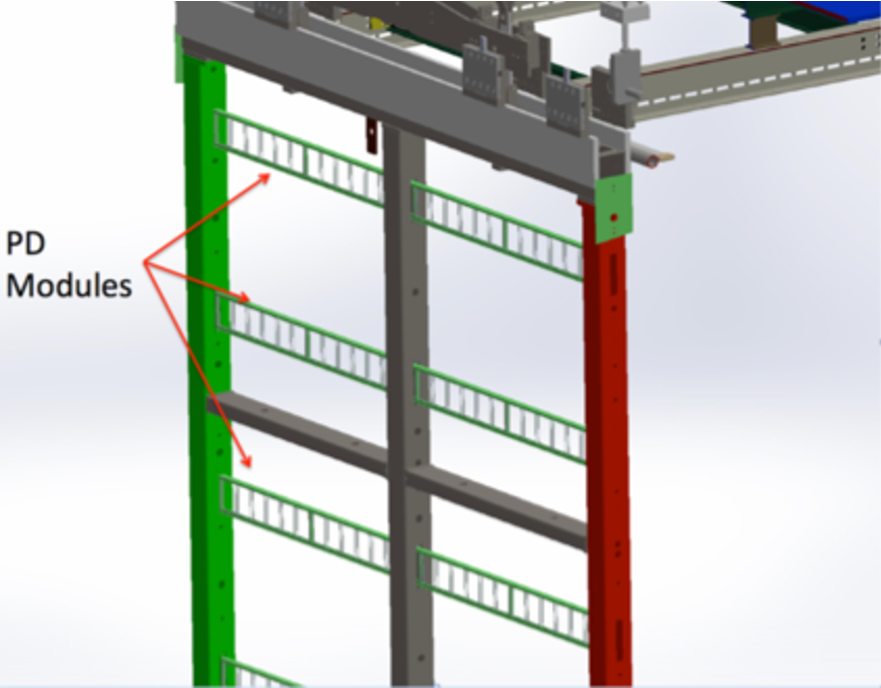
\includegraphics[width=0.49\textwidth]{PDsInAPA.pdf}
\end{dunefigure}

Photon-detector modules, shown in Figure~\ref{fig:PDModules}, are $\SI{209.2}{\cm}\times\SI{11.8}{\cm}\times\SI{2.3}{\cm}$ bars, ten of which are mounted in each APA, inside the wire layers. Each bar contains 24 X-Arapuca\footnote{An arapuca is a South American bird trap, the name used here in analogy to the way the X-Arapuca devices trap photons.} cells, grouped into four supercells. An X-Arapuca cell is shown in Figure~\ref{fig:ArapucaCell}. The outer layers are dichroic filters that are transparent to the \SI{126.8}{\nano\meter} scintillation light. Between these filters is a wavelength-shifting (WLS) plate, which converts the photons into the visible spectrum.
%; one WLS plate runs the full length of one supercell.
Visible photons emitted inside the WLS plate at an angle to the surface greater than the critical angle are transported to SiPMs at the ends of the plates. Visible photons that escape the WLS plates are reflected off the dichroic filters, which have an optical cutoff for photons with wavelengths above \SI{400}{\nano\meter}, back into the WLS plates. 

\begin{dunefigure}[An X-Arapuca photon-detector cell.]{fig:ArapucaCell}
{Left: an X-Arapuca cell. Right: an exploded view of the X-Arapuca cell, where the blue sheet is the wavelength-shifting plate and the yellow sheets the dichroic filters.}
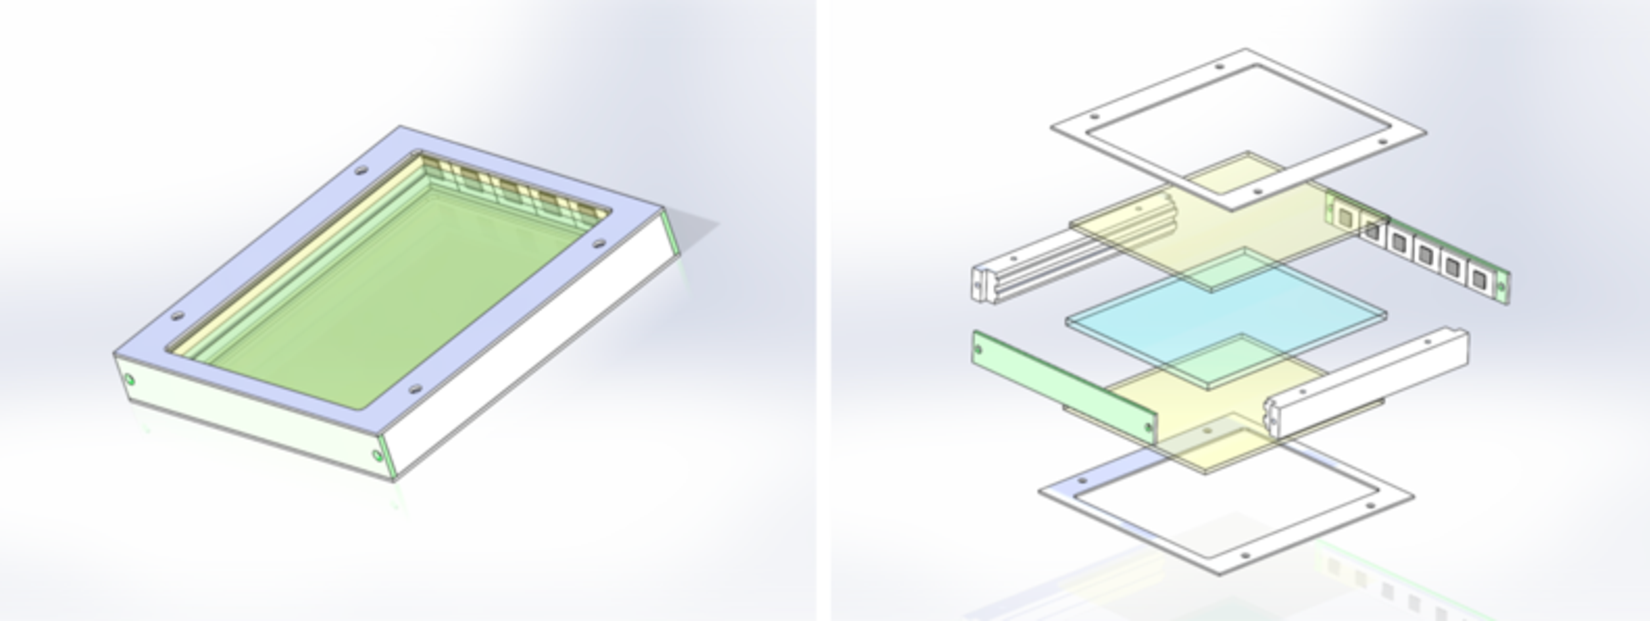
\includegraphics[width=\textwidth]{XArapuca.pdf}
\end{dunefigure}

The 48 SiPMs on each X-Arapuca module are ganged together and the signals collected by front-end electronics, mounted on the module, the design of which is inspired by the system used for the Mu2e cosmic-ray tagger, which uses commercial ultrasound ASICs. This front-end electronics defines the \SI{1}{\micro\second} timing resolution of the photon-detector system.

\section{High voltage}
\label{sec:fdsp-exec-hv}

The design voltage at which the DUNE TPC will operate is $-\SI{180}{\kilo\volt}$, corresponding to \SI{500}{\volt/\cm} accross each drift volume. This voltage is chosen as a trade-off between the fact that a higher voltage results in more charge collected, and hence better signal-to-noise ratio, better calorimetry and lower detection thresholds, and also less saturation of free charge at the point of ionisation, but that a higher voltage also reduces the amount of scintillation light produced and requires a greater space between the CPAs and the field cage, reducing the fiducial volume. The ProtoDUNE experience has shown that we can achieve this design voltage; nevertheless, from MicroBooNE we know that a drift voltage of \SI{250}{\volt/\cm} achieves an adequate signal-to-noise ratio.

The high voltage is supplied to the CPA arrays. Each CPA array (two per \SI{10}{\kilo\tonne} module) has its own independent high-voltage supply. The high-voltage supplies are commercial devices that will supply a current of \SI{0.16}{\milli\ampere} at $-\SI{180}{\kilo\volt}$. The voltage is delivered, via $\sim\!\SI{30}{\meter}$ length commercial cables, through a series of few-\si{\mega\ohm} filtering resistors that act as low-pass filters to reduce noise to satisfy the ripple-voltage requirement of $<\!\SI{0.9}{\milli\volt}$ on the CPA array, which corresponds to a requirement of $<\!100\,e-$ of noise injected into the TPC by the high-voltage system. The supply unit monitors the voltage and current every \SI{300}{\milli\second}; toroids mounted on the cables are senstive to much faster changes in current and enable response to current changes on a \SIrange{0.1}{10}{\micro\second} timescale.

The high-voltage passes into the cryostat through a feedthrough based on the ICARUS design~\cite{ref:ICARUSFeedthrough}, %Reference [6] in the HV chapter
the stainless steel conductor of which mates with the CPA array via a spring-loaded feedthrough.

When at $-\SI{180}{\kilo\volt}$, each CPA array stores \SI{400}{\joule} of energy, and therefore the CPAs must have at least $\SI{1}{\mega\ohm/\cm^{2}}$ resistance to prevent damage if the field is quenched. The CPA, one of which is shown in Figure~\ref{fig:CPA}, is a $\SI{1.2}{\meter}\times\SI{2}{\meter}$ planar unit, each side of which is a \SI{3}{\mm} thick FR-4 sheet, onto which is laminated a thin layer of carbon-impregnated Kapton that forms the resistive cathodic plane.

\begin{dunefigure}[A cathode plane assembly.]{fig:CPA}
{A cathode plane assembly.}
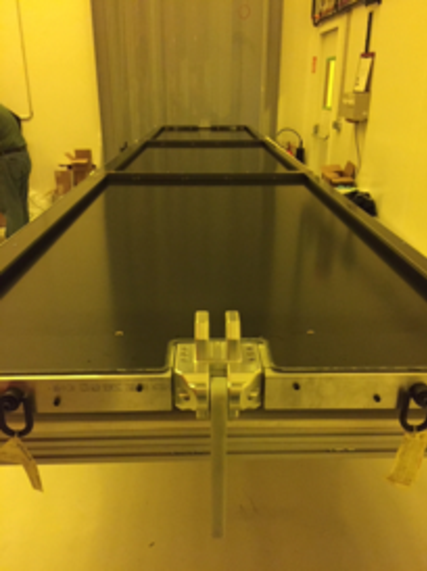
\includegraphics[width=0.35\textwidth]{CPA.pdf}
\end{dunefigure}

The field must be uniform, throughout the active TPC volume, to within 1\%, and this is achieved by a field cage that surrounds the drift volumes. The field cage is built from field-shaping aluminimum profiles, terminated with \SI{6}{\mm} thick ultra-high molecular-weight polyethylene caps, as shown in Figure~\ref{fig:FieldCage}. It is vital that all surfaces on these profiles are smooth to keep local fields below \SI{30}{\kilo\volt/\cm}, a requirement that reduces the possibility of voltage breakdowns in the argon; the shape of the profiles chosen leads to a maximum local field near the surface of the field cage of $\sim\!\SI{12}{\kilo\volt/\cm}$. The aluminium profiles are connected together via a resistive divider chain; between each profile, two \SI{5}{\giga\ohm} resistors, arranged in parallel, provide a \SI{2500}{\mega\ohm} resistance to create a nominal \SI{3}{\kilo\volt} drop.

\begin{dunefigure}[A section of the field cage.]{fig:FieldCage}
{A section of the field cage, showing the extruded aluminium field-shaping profiles.}
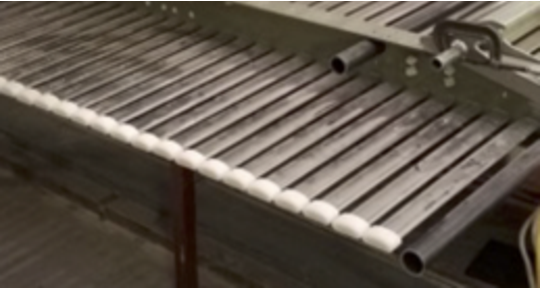
\includegraphics[width=0.5\textwidth]{FieldCage.pdf}
\end{dunefigure}

\section{Anode planes}
\label{sec:fdsp-exec-apas}

The anode plane assemblies (APAs) are $\SI{6}{\meter}\times\SI{2.3}{\meter}$ planes that form the three anodic walls of the TPC: two along the edges and one down the middle, as shown in Figure~\ref{fig:DUNESchematic}. An APA is shown in Figure~\ref{fig:APA}. In the Far Detector, the APAs are mounted in pairs, in portrait orientation, one above another, with the head end of the top APA at the top of the detector and the head end of the bottom APA at the bottom of the detector.

\begin{dunefigure}[An anode plane assembly.]{fig:APA}
{Top: a schematic of an anode plane assembly. Bottom: a ProtoDUNE anode plane assembly. The right-hand end of the APA as shown in this picture is the head end, onto which the cold electronics is mounted (the blue boxes in the upper picture). }
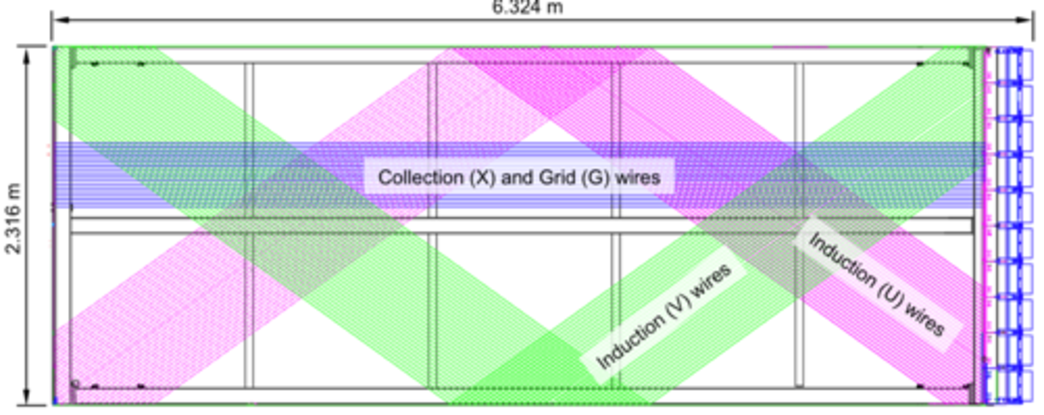
\includegraphics[width=0.7\textwidth]{APASchematic.pdf}
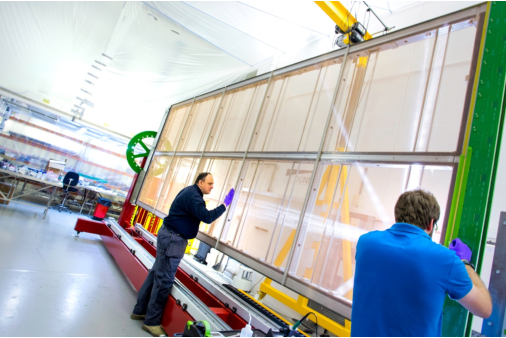
\includegraphics[width=0.6\textwidth]{RealAPA.pdf}
\end{dunefigure}

The basic building block of the APA is the $\SI{6}{\meter}\times\SI{2.3}{\meter}$ steel frame that can be seen outlined in Figure~\ref{fig:APA}, consisting of three long sections, a head shaft onto which the cold electronics is mounted, a foot shaft, and four thinner cross-braces. The two outer long sections are $4\,\mathrm{inch}\times 4\,\mathrm{inch}$ square-profile steel tubes through which the photon-detector cables, and the cold-electronics cables from the bottom APA of a pair, run. The photon detectors are mounted into the APAs, after production, through slots in these long sections.

Mounted directly onto both sides of the APA frame is a grounding mesh, which ensures any ionisation produced in the APA cannot cause signals on the active wire layers. Around this are wound the four wire layers, consisting of \SI{150}{\micro\meter} diameter copper-beryllium wire. The inside layer is the collection layer, called the $x$-layer, the 960 wires of which run parallel to the long axis of the APA. Next are the two induction layers, the $u$- and $v$-layers, each with 800 wires at \SI{35.7}{\degree} to the long axis. Finally, the uninstrumented shielding layer, the $g$-layer, has 960 wires running parallel to the $x$-layer wires and exists to shield the three active layers from long-range induction effects. The wire spacing on each layer is close to \SI{5}{\mm}, and the inter-plane spacing is \SI{4.75}{\mm}. The $\sim\!\SI{5}{\mm}$ spacing on each plane defines the spacial resolution of the APA; it is wide enough to keep readout costs low and signal-to-noise high but small enough to enable reconstruction of short tracks such as few-\si{\cm} kaon tracks from proton-decay events. The tolerance both on the wire spacing in the plane and on the plane-to-plane spacing is \SI{0.5}{\mm}; this is most important in the plane-to-plane direction where the spacing ensures that the induction planes remain transparent to the drifting charge.

Around the four sides of the APA are printed circuit boards called geometry boards to which the wires are soldered, so-called since these boards define the wire spacing in all dimensions. These boards, shown in Figure~\ref{fig:GeometryBoardsAndCombs}, consist only of pads and traces: no active components. At the head end, these boards lie flat in the plane of the APA, and the wires are terminated onto these boards for readout. On the remaining three sides, the boards sit on the sides of the APA, perpendicular to the wire planes, and are used to control the wrapping of the wires around the APA. These wrap boards have insulating pins on their edges, around which the wires are wrapped, to set the wire spacing. At the head end, additional, active boards are installed after all wires are wound: $g$-bias boards provide the necessary capacitance to the $g$-layer and a resistor to provide the bias voltage; $CR$-boards provide the interface between the $x$ and $u$ layers and the cold electronics, resistors providing the bias voltages and capacitors providing DC-blocking. Relative to the ground the four wire layers are biased to \SI{820}{\volt} ($x$-layer), \SI{0}{\volt} ($v$-layer), \SI{-370}{\volt} ($u$-layer) and \SI{-665}{\volt} ($g$-layer). To maintain the wire spacing across the APA, wire-support combs, also shown in Figure~\ref{fig:GeometryBoardsAndCombs}, run along the four cross-braces across the short dimension of the APA.

\begin{dunefigure}[Geometry boards and wire-support combs on an anode plane assembly.]{fig:GeometryBoardsAndCombs}
{Left: geometry boards, showing the head-end boards face-on and the wrap boards along the bottom. Back plastic teeth are visible on the edges of the wrap boards. Right: wire-support combs.}
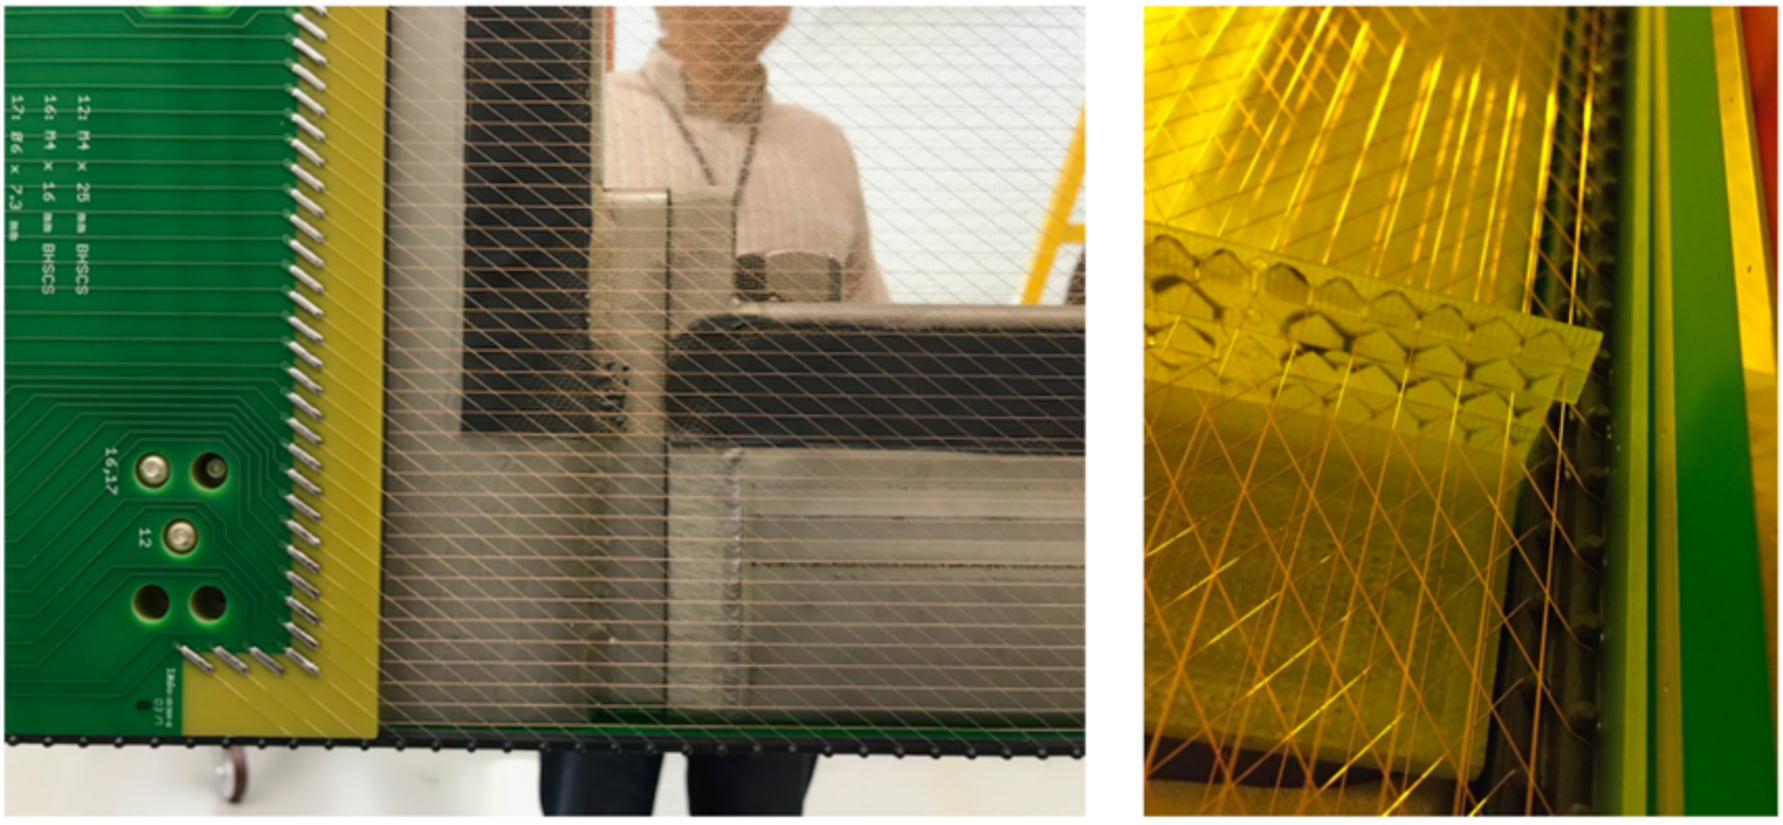
\includegraphics[width=\textwidth]{GeometryBoardsAndCombs.pdf}
\end{dunefigure}

In the Far Detector, APAs are hung in pairs, one above another, the bottom APA hanging from the top APA. Each APA must be electrically isolated from all its neighbours, and so the mechanical linkages are made using parts made from G10.

%COMMENT note that I haven't talked at all about construction throughout this chapter.

\section{Electronics}
\label{sec:fdsp-exec-electronics}

The job of the readout electronics is to send out of the cryostat digitized waveforms from the APA wires. To enable us to look at low-energy particles, we aim to keep noise to below $1000\,e^{-}$ per channel, which should be compared to the $20k$--$30k\,e^{-}$ per channel from a minimum-ionizing particle. For large signals, we require a linear response up to $500,000\,e^{-}$, which ensures that fewer than 10\% of beam events experience saturation. This can be achieved using 12\,ADC bits. In addition, the electronics are designed with a front-end peaking time of \SI{1}{\micro\second}, which matches the time for the electrons to drift between wires planes on the APA; this then leads to a design sampling frequency of \SI{2}{\mega\hertz}.

The digitization electronics are mounted on the head ends of the APAs, in the liquid argon, and are therefore referred to as cold electronics. The low temperatures result in a reduction in thermal noise. A block diagram of the front-end motherboards that are mounted on the APAs is shown in Figure~\ref{fig:ElectronicsBlockDiagram}. Each APA is instrumented with 20 front-end motherboards, each of which take the signals from 40 $u$-layer wires, 40 $v$-layer wires and 48 $x$-layer wires. The signals all pass through a series of three ASICs. The first ASIC, the front-end ASIC, shapes and amplifies the signals. The next ASIC, the ADC ASIC, performs the analogue-to-digital conversion. Finally, a COLDATA ASIC merges the datastreams from the preceding ASICS for transmission to the outside world; this COLDATA ASIC also controls the front-end motherboard and facilitates communications between the motherboard and the outside world.

\begin{dunefigure}[A block diagram of the anode-plane readout electronics.]{fig:ElectronicsBlockDiagram}
{A block diagram of the readout electronics mounted on the APAs.}
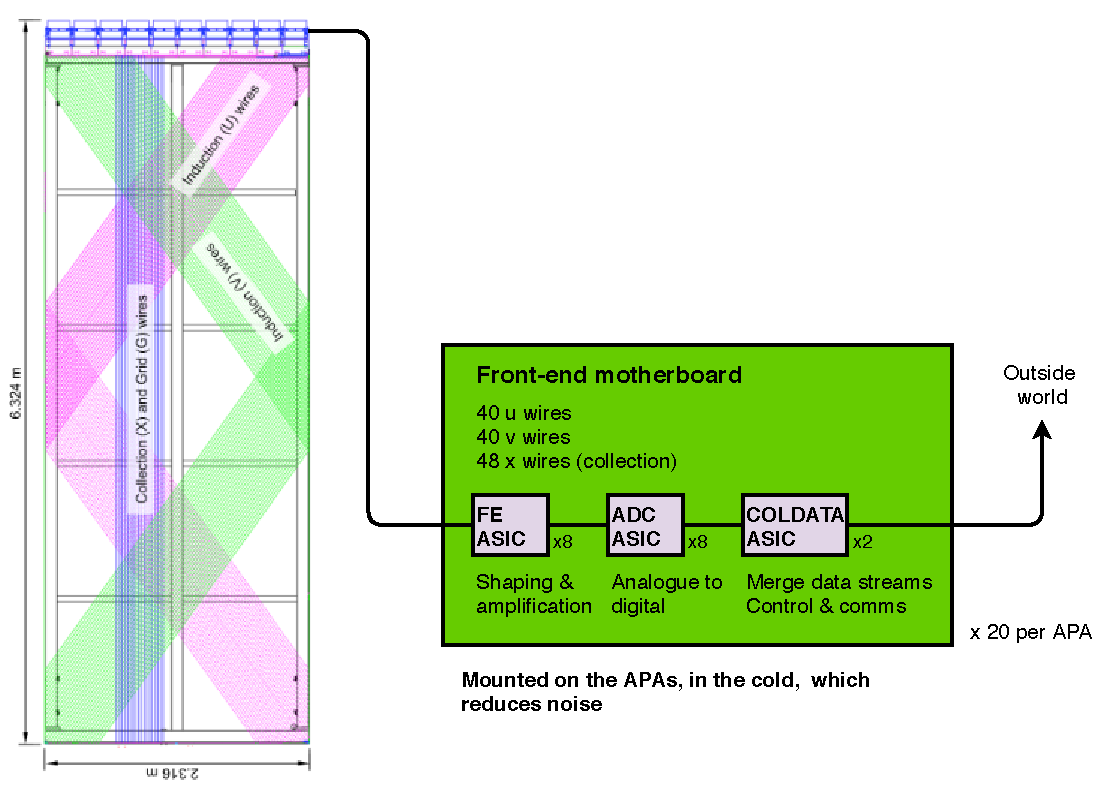
\includegraphics[width=0.8\textwidth]{ElectronicsBlockDiagram.pdf}
\end{dunefigure}

Once the data has passed out of the cryostat, through feedthroughs in the roof, it is passed to warm interface boards, which transmit the signals to the data-acquisition system along \SI{10}{\giga\byte/\second} optical fibres. These warm interface boards also transmit the clock and control signals, and low-voltage power, back to the front-end motherboards.

\section{Data acquisition}
\label{sec:fdsp-exec-daq}

The data-acquisition system (DAQ) is located underground, in the central utility cavern, adjacent to the main detector caverns. It is based on the CERN-designed FELIX system used for the LHC experiments. Each \SI{10}{\kilo\tonne} module has its own independent DAQ system. The DAQ must be able to independently trigger the TPC readout for all event types, including beam events, nucleon-decay events and supernova bursts.

The supernova burst provides the DAQ with the greatest challenge. Here, the DAQ must, with zero dead-time, be able to trigger on interactions below \SI{100}{\mega\electronvolt} spaced over many seconds, throughout the detector volume. The target for doing this is $>\!90\%$ efficiency for each \SI{10}{\kilo\tonne} module for supernovae within \SI{100}{\kilo\parsec}; once triggered, a module will then send a trigger signal through to the other three modules. The DAQ must then handle the immense data-rate involved: the entire detector must be read out for up to \SI{100}{\second}, including a \SI{4}{\second} pre-trigger window; the full data-rate from a module can be as high as \SI{2}{\tera\byte/\second}. For beam events and nucleon-decay events, the problem is much simpler as only a localised part of the detector around the event need be read out, and the read-out window only needs to be of the order of the length of a drift window: around \SI{30}{\milli\second}.

The 150 APAs from each \SI{10}{\kilo\tonne} module are processed by 75 FELIX boards. The photon detectors from the module will have a lower data-rate, and so will be processed by 6--8 additional FELIX boards. Each FELIX board sits below ground in its own host server, and talks to a data-selection server which may be either above or below ground. The data is finally transferred to Fermilab over network, and we aim to ensure we achieve a data-rate to tape of less than \SI{30}{\peta\byte/\year}.

The DAQ must also provide the system clock that keeps the detector components synchronised and timestamps all the data. The timestamp derives from a GPS pulse-per-second that is fed into the DAQ with \SI{1}{\micro\second} precision, adequate precision to timestamp beam and supernova events. To provide the finer synchronisation between detector components, a \SI{10}{\mega\hertz} reference clock drives the module's \SI{65}{\mega\hertz} masterclock, which is fanned out to all detector components, providing an overall synchronisation to a precision of \SI{1}{\nano\second}.

\section{Conclusion}
\label{sec:fdsp-exec-conclusion}

The chapters that follow go into significantly more detail about the design of the \SI{10}{\kilo\tonne} single-phase far-detector modules. In addition to describing the design and requirements, these chapters include details on the construction procedures, quality-control procedures, and the way in which the design has been validated and informed by ProtoDUNE.

